\section{Quantile Regression based time series model}

Let the $\alpha$-conditional quantile function of $Y$ for a given value $x$ of the $d$-dimensional random variable $X$, i.e., $Q_{Y|X}:[0,1] \times \mathbb{R}^d \rightarrow \mathbb{R}$, can be defined as %(in short, from now on, $Q_{Y|X}(\cdot, \cdot)$)
\begin{equation}
Q_{Y|X}(\alpha,x) = F_{Y|X}^{-1}(\alpha,x) = \inf\{y: F_{Y|X}(y,x) \geq \alpha\}.
\label{eq:quantile-function}
\end{equation}
Let a dataset be composed of $n$ observations of $\{y_t,x_t \}_{t=1}^n$. The sample quantile function is based on a finite number of observations and is the solution to the following optimization problem:
\begin{eqnarray}
\hat{Q}_{Y|X}(\alpha,\cdot)\quad\in\quad & \underset{q_{\alpha}}{\text{arg min}}\, & \sum_{t\in T}\rho_{\alpha}(y_{t}-q_{\alpha}(x_t)),\label{eq:optim-lqr1} \\
 & q_{\alpha}\in\mathcal{Q}.\label{eq:optim-lqr2}
\end{eqnarray}
where $\rho$ is the check function, defined as
\begin{equation}\label{eq:check-function}
\rho_{\alpha}(x)=\begin{cases}
\alpha x & \text{if }x\geq0\\
(1-\alpha)x & \text{if }x<0
\end{cases}.
\end{equation}
Quantile $q_\alpha$ belongs to a function space $\mathcal{Q}$. We might have different assumptions for space $\mathcal{Q}$, depending on the type of function we want to find for $q_\alpha$. A few properties, however, must be achieved by our choice of space, such as being continuous and having limited first derivative. In this paper, we consider the case where $\mathcal{Q}$ is a linear function's space.

The problem (\ref{eq:optim-lqr1})-(\ref{eq:optim-lqr2}) can be rewritten as a Linear Programming problem as in (\ref{eq:linear-opt-1})-(\ref{eq:linear-opt-ult}), thus being able to use a modern solver to fit our model. Variables $\varepsilon^+_t$ e $\varepsilon^-_t$ represent the quantities $|y-q(\cdot)|^+$ and $|y-q(\cdot)|^-$, respectively. $A$ is the set containing a sequence of probabilities  $\alpha_i$ such that $0 < \alpha_1 < \alpha_2 < \dots < \alpha_Q < 1$. This set represents a finite discretization of the interval $[0,1]$.  
\begin{IEEEeqnarray}{lr}
\min_{\beta_{0\alpha},\beta_\alpha,\varepsilon_{t\alpha}^{+}, \varepsilon_{t\alpha}^{-}} \, \sum_{\alpha \in A} \sum_{t \in T}\left(\alpha \varepsilon_{t \alpha}^{+}+(1-\alpha)\varepsilon_{t \alpha}^{-}\right) \span \label{eq:linear-opt-1}\\
\mbox{s.t. } \span \nonumber \\
\varepsilon_{t \alpha}^{+}-\varepsilon_{t \alpha}^{-}=y_{t} - \beta_{0\alpha} - \beta_{\alpha}^T x_{t}, & \forall t \in T,\forall \alpha \in A, \\
\varepsilon_{t\alpha}^+,\varepsilon_{t\alpha}^- \geq 0, &  \forall t \in T,\forall \alpha \in A,\\ 
\beta_{0\alpha} + \beta_{\alpha}^T x_{t} \leq \beta_{0\alpha'} + \beta_{\alpha'}^T x_{t}, \span \nonumber \\
\label{eq:linear-opt-ult} \forall t \in T, \forall (\alpha, \alpha') \in A \times A,  \alpha < \alpha',
\end{IEEEeqnarray}
After solving the problem, the sequence $\{ q_\alpha \}_{\alpha \in A}$ is fully defined by the optimum values $\beta^*_{0\alpha}$ and $\beta^*_\alpha$, for every $\alpha$.

We apply QR to estimate the conditional distribution $\hat{Q}_{Y_{t+k}|X_{t+k},Y_t, Y_{t-1}, \dots} (\alpha,\cdot)$ for a $k$-step ahead forecast of time serie $\{y_t\}$, where $X_{t+k}$ is a vector of exogenous variables at the time we want to forecast. Once the conditional distribution is estimated, we are able to simulate and generate scenarios. In the next session, regularization techniques are presented, in order to choose parsimoniously which variables will be input for $\hat{Q}$.

%Let $A$ be a set containing a sequence of probabilities  $\alpha_i$ such that $0 < \alpha_1 < \alpha_2 < \dots < \alpha_Q < 1$. This set represents a finite discretization of the interval $[0,1]$.
%One of our goals with quantile regression is to estimate a quantile function $\hat{Q}_{Y|X}$ of a given real valued random variable $X$ from a sequence of quantiles $q_{\alpha_1}(x_t) \leq q_{\alpha_2}(x_t) \leq \dots \leq q_{\alpha_{|A|}}(x_t)$, with $0 < \alpha_1 < \alpha_2 < \dots < \alpha_{|A|} < 1$, for any given $t$.
%The process of fitting $\hat{Q}_{Y|X}$ is by mapping every $\alpha_i$ with its estimated quantile $\hat{q}_{\alpha_i}(x_t)$.
%The denser the grid of values in $A$, better is the approximation of $Q_{Y|X}$.
%Thus, the distribution found for $Y$ is nonparametric, as no previous assumptions are made about its shape, and its form is fully recovered by the data we have.
%
%The crossing quantile is a common issue when estimating a set of quantiles \cite{chernozhukov_quantile_2010}. Two a solution may be 
%
%
%A typical problem, however, arises when working with quantile regression. When quantiles are estimated independently, it is possible to find $q_{\alpha}(x_t) > q_{\alpha'}(x_t)$, for a given $t$, when $\alpha_1 < \alpha_2$. An example can be seen on Figure \ref{fig:crossing-quantiles}, where quantiles $\alpha = 0.95$ and $\alpha = 0.9$ cross. This problem, called \textit{crossing quantiles}, can be prevented by estimating all quantiles with a single minimization problem.
%
%
%
%As opposed to traditional parametric models where one has to assume the error distribution on the model
%\begin{equation}
%y_t = h(F_t) + \varepsilon_t,
%\end{equation}
%as we choose the nonparametric methodology we are released from this step. A distribution for $\varepsilon_t$ is defined within the estimation procedure. The predictive distribution is derived from the individual quantiles
%\begin{equation}
%\hat q^\alpha_{t+k|k} = \hat y_{t+k|t} + \hat F^\varepsilon_{t,k}(\alpha).
%\end{equation}
%% % coisas aqui % %
%\cite{wan_direct_2017} defines a model based on extreme machine learning to estimate every $\alpha$-quantile in a thin grid $0 < \alpha_1 < \alpha_2 < \dots < \alpha_Q < 1$. 
%	
%	
%	
%	
%	
%	
%%\subsection{Linear parametric explanatory model}
%%	\blindtext
%
%One of the options is to consider function $q_\alpha(\cdot)$ in problem (\ref{eq:optim-qr1})-(\ref{eq:optim-qr2}) as a linear function of its parameters. In this setup, 
%\begin{equation}
%\hat q_\alpha(x_t) = \beta^T x_t + \beta_0.
%\end{equation}
%
%\section{Regularization}
%Our study also (...) the regularization process together with the estimation of the conditional distribution function, which is a contribution in this paper.
%
%We investigate two ways of regularization.
%The first of them consists of selecting the best subset of variables through Mixed Integer Programming, given that $K$ variables are included in the model. 
%
%The second way is including a $\ell_1$ penalty on the linear quantile regression, 
%Both of them will be built over the standard Quantile Linear Regression model. In the end of the section, we discuss a information criteria to be used for quantile regression and verify how close are the solutions in the eyes of this criteria.
%
%When we choose $q_\alpha(x_t)$ to be a linear function
%\begin{equation}
%\hat{q}_\alpha(x_t) = \beta_{0\alpha} + \beta_\alpha^T x_t 
%\end{equation}
%we can substitute it on problem \ref{eq:qar-general}, getting the following LP problem:

	
	
%To model \ref{eq:linear-model} as a Linear Programming problem, thus being able to use a modern solver to fit our model,  we create variables $\varepsilon^+_t$ e $\varepsilon^-_t$ to represent the positive and the negative values of \ref{eq:check-function}, respectively. The optimal argument $q_\alpha^*(\cdot)$ on the Linear Programming problem \ref{eq:qar-general} is the estimated $\alpha$-quantile for the given random sample.
%\begin{equation}
%\begin{aligned}q^*_\alpha(.) \in \underset{q_\alpha (\cdot),\varepsilon_{t}^{+}, \varepsilon_{t}^{-}}{\text{arg min}} & \sum_{t \in T}\left(\alpha \varepsilon_{t}^{+}+(1-\alpha)\varepsilon_{t}^{-}\right) & \\
%\mbox{s.t. } & \varepsilon_{t}^{+}-\varepsilon_{t}^{-}=y_{t}-q_\alpha(x_t), & \qquad\forall t \in T,\\
%& \varepsilon_t^+,\varepsilon_t^- \geq 0, & \qquad \forall t \in T.
%\end{aligned}
%\label{eq:qar-general}
%\end{equation}
%
%	
%\subsection{General non-linear nonparametric model}
%	\blindtext
%	
%A quantile of a random variable is important in risk measuring, as we can measure the probability of occurrence of extreme events, and in many other fields. While working with energy forecasts, quantile regression can produce interesting results when working with both short term (hourly) or long term (monthly) data. As an example, we present a solar time series for the short term and a wind time series for long term. The first set of data is measured at the location of Tubarao (Brazil) on the year of 2014, while the latter is a dataset of mean power  monthly observations from Icaraizinho (Brazil) between 1981 to 2011 of measured in Megawatts. Figure \ref{fig:boxplots} illustrate the seasonality present in these datasets.
%
%\begin{figure}
%	\centering
%	\begin{minipage}[t]{\linewidth}
%		
%		\begin{minipage}[t]{0.45\linewidth}
%			%\centering
%			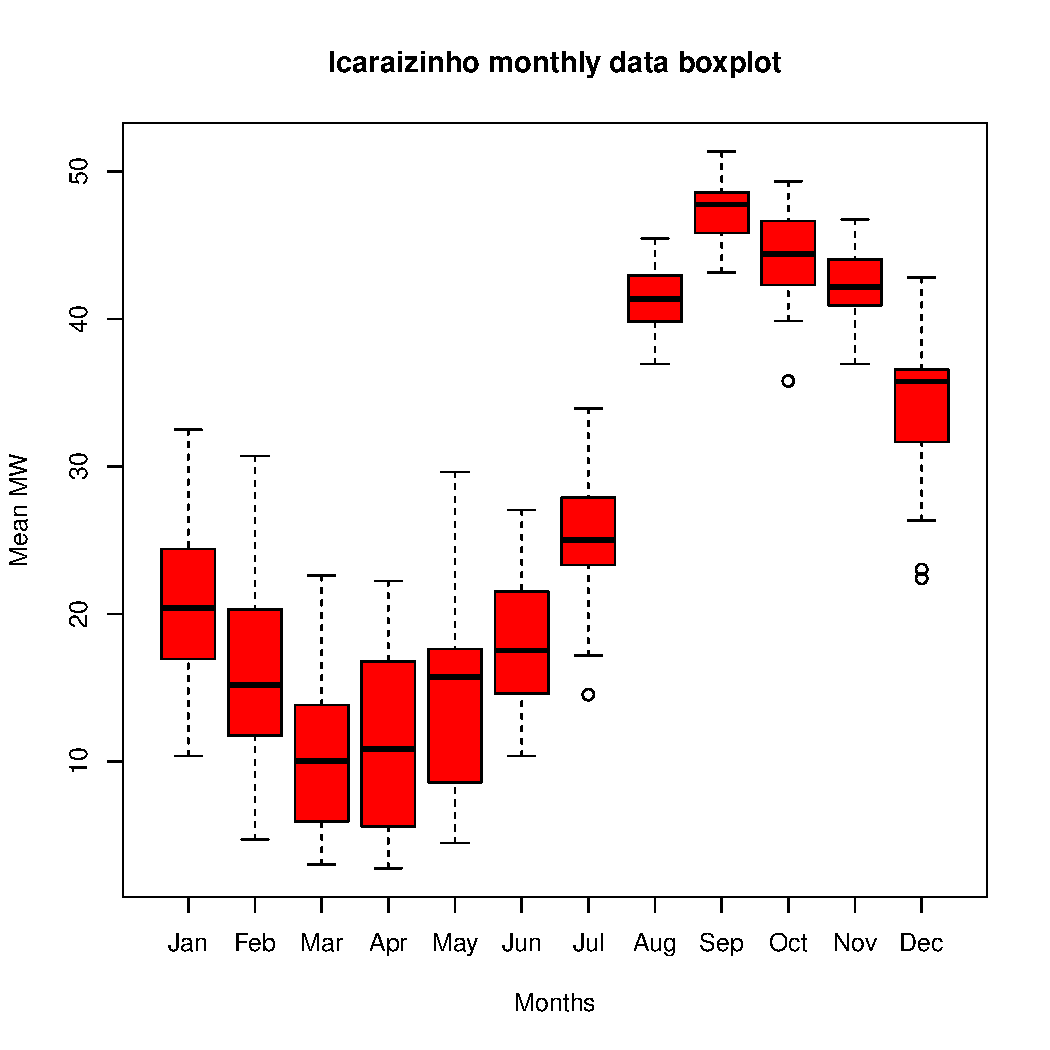
\includegraphics[width=\textwidth]{./../Figuras/Icaraizinho/icaraizinho-boxplot}
%			%\caption{Boxplot for each month for the Icaraizinho dataset}
%			\label{fig:icaraizinho-boxplot}
%		\end{minipage}
%		\begin{minipage}[t]{0.45\linewidth}
%			%\centering
%			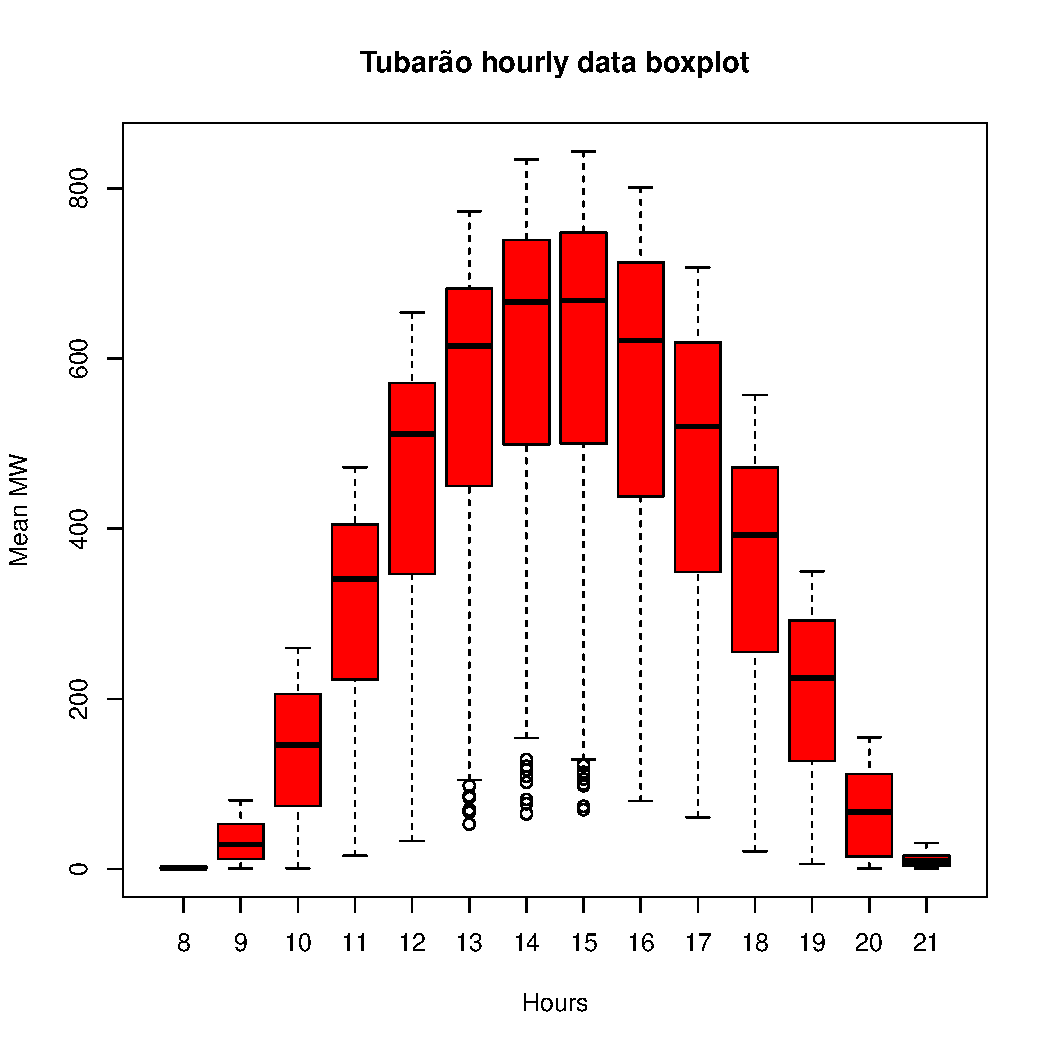
\includegraphics[width=\textwidth]{./../Figuras/Solar-exemplos/tubarao-boxplot}
%			%\caption{Boxplot for each month for the Icaraizinho dataset}
%			\label{fig:tubarao-boxplot}
%		\end{minipage}
%	\end{minipage}
%	\caption{Boxplots showing seasonality for monthly and hourly data.}
%	\label{fig:boxplots}
%\end{figure}

